\tikzset{every picture/.style={line width=0.75pt}} %set default line width to 0.75pt

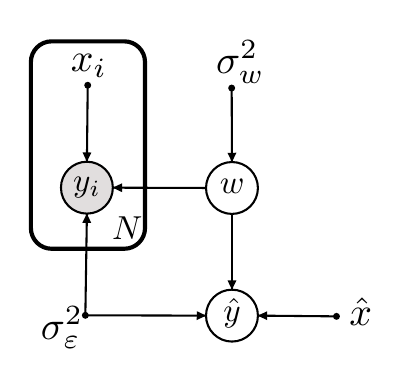
\begin{tikzpicture}[x=0.75pt,y=0.75pt,yscale=-0.5,xscale=0.5]
%uncomment if require: \path (0,350); %set diagram left start at 0, and has height of 350

\draw    (208.5,285) -- (210,187) ;
\draw [shift={(210,187)}, rotate = 450.88] [fill={rgb, 255:red, 0; green, 0; blue, 0 }  ] [draw opacity=0] (8.93,-4.29) -- (0,0) -- (8.93,4.29) -- (8.93,-4.29)    ;
\draw [shift={(208.5,285)}, rotate = 270.88] [fill={rgb, 255:red, 0; green, 0; blue, 0 }  ] [draw opacity=0]    (0, 0) circle [x radius= 3.35, y radius= 3.35]   ;
\draw    (349.78, 162.29) circle [x radius= 25, y radius= 25]  ;
\draw  [fill={rgb, 255:red, 225; green, 222; blue, 222 }  ,fill opacity=1 ]  (210, 162) circle [x radius= 25, y radius= 25]  ;
\draw    (324.78,162.29) -- (235,162) ;
\draw [shift={(235,162)}, rotate = 360.18] [fill={rgb, 255:red, 0; green, 0; blue, 0 }  ] [draw opacity=0] (8.93,-4.29) -- (0,0) -- (8.93,4.29) -- (8.93,-4.29)    ;

\draw  [line width=1.5]  [rounded corners= 7.5] (156, 21) rectangle (266, 220.86)   ;
\draw    (349.5,66) -- (349.78,137.29) ;
\draw [shift={(349.78,137.29)}, rotate = 269.77] [fill={rgb, 255:red, 0; green, 0; blue, 0 }  ] [draw opacity=0] (8.93,-4.29) -- (0,0) -- (8.93,4.29) -- (8.93,-4.29)    ;
\draw [shift={(349.5,66)}, rotate = 89.77] [fill={rgb, 255:red, 0; green, 0; blue, 0 }  ] [draw opacity=0]    (0, 0) circle [x radius= 3.35, y radius= 3.35]   ;
\draw    (210.78,63.29) -- (210,137) ;
\draw [shift={(210,137)}, rotate = 270.61] [fill={rgb, 255:red, 0; green, 0; blue, 0 }  ] [draw opacity=0] (8.93,-4.29) -- (0,0) -- (8.93,4.29) -- (8.93,-4.29)    ;
\draw [shift={(210.78,63.29)}, rotate = 90.61] [fill={rgb, 255:red, 0; green, 0; blue, 0 }  ] [draw opacity=0]    (0, 0) circle [x radius= 3.35, y radius= 3.35]   ;
\draw    (349.78, 285.29) circle [x radius= 25, y radius= 25]  ;
\draw    (208.5,285) -- (324.78,285.29) ;
\draw [shift={(324.78,285.29)}, rotate = 180.14] [fill={rgb, 255:red, 0; green, 0; blue, 0 }  ] [draw opacity=0] (8.93,-4.29) -- (0,0) -- (8.93,4.29) -- (8.93,-4.29)    ;

\draw    (349.78,187.29) -- (349.78,260.29) ;
\draw [shift={(349.78,260.29)}, rotate = 270] [fill={rgb, 255:red, 0; green, 0; blue, 0 }  ] [draw opacity=0] (8.93,-4.29) -- (0,0) -- (8.93,4.29) -- (8.93,-4.29)    ;

\draw    (450.5,286) -- (374.78,285.29) ;
\draw [shift={(374.78,285.29)}, rotate = 360.53999999999996] [fill={rgb, 255:red, 0; green, 0; blue, 0 }  ] [draw opacity=0] (8.93,-4.29) -- (0,0) -- (8.93,4.29) -- (8.93,-4.29)    ;
\draw [shift={(450.5,286)}, rotate = 180.54] [fill={rgb, 255:red, 0; green, 0; blue, 0 }  ] [draw opacity=0]    (0, 0) circle [x radius= 3.35, y radius= 3.35]   ;

\draw (210,162) node [scale=1.2]  {$y_{i}$};
\draw (249,201) node [scale=1.2]  {$N$};
\draw (186,297) node [scale=1.44]  {$\sigma ^{2}_{\varepsilon }$};
\draw (358,41) node [scale=1.44]  {$\sigma ^{2}_{w}$};
\draw (212,45) node [scale=1.44]  {$x_{i}$};
\draw (474,281) node [scale=1.44]  {$\hat{x}$};
\draw (350,283) node [scale=1.2]  {$\hat{y}$};
\draw (350,161) node [scale=1.2]  {$\boldsymbol{w}$};


\end{tikzpicture}
